\section{Discrete-Time Signals and Systems}
\subsection{Discrete-Time Signals}
A discrete-time signal is mathematically represented
as a sequence of data. The
sequence $x$ contains the numbers indexed by
the discrete-time integer $n$:
\[
    x = \{ x[n] \}, \quad -\infty < n < \infty
\]
Any arbitrary sequence can be expressed as the sum of scaled and delayed impulses:
\[
    x[n] = \sum_{k=-\infty}^{+\infty} x[k] \delta[n-k]
\]
where $\delta[n-k]$ is the shift of the unit impulse sequence $\delta[n]$ (Kronecker delta), defined as
\[
    \delta[n] = 
    \begin{cases}
        0,  & n \neq 0 \\
        1,  & n = 0
    \end{cases}
\]

%==================================
\subsection{Discrete-Time Systems}
\begin{figure}[H]
    \centering
    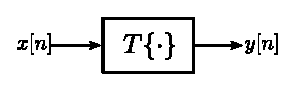
\includegraphics[width=.4\textwidth]{images/discrete-time-system.eps}
    \caption{Representation of a discrete-time system. $T\{\cdot\}$ is a transformation operator that maps an input sequence $x[n]$ into an output sequence $y[n]$.}
    \label{fig:dt_sys}
\end{figure}

\begin{ex}{The Moving Average System}
The moving average system is a discrete-time system. It is defined as
\begin{align*}
    y[n] 
    & = \frac{1}{M_1 + M_2 + 1} \sum_{k=-M_1}^{M_2} x[n-k] \\
    & = \frac{1}{M_1 + M_2 + 1} (x[n+M_1] + x[n+M_1 -1] + ... + x[n] + x[n-1] + x[n-M_2])
\end{align*}
The system computes the $n$\textsuperscript{th} sample of the output sequence as the average of $(M_1+M_2+1)$ samples of the input sequence around the $n$\textsuperscript{th} sample.
\end{ex}
%==================================
\subsubsection{Memoryless Systems}
A system is \textit{memoryless} if the system output $y[n]$ at every value of $n$ depends only on the input $x[n]$ at the same value of $n$.
\begin{ex}{A Memoryless System}
    \[
        y[n] = (x[n])^2, \quad \text{for each value of $n$.}
    \]
\end{ex}
%==================================
\subsubsection{Linear Systems}
A system is \textit{linear} if and only if
\[
    T\{ x_{1}[n] + x_{2}[n] \} 
    =  T\{ x_{1}[n] \} + T\{ x_{2}[n] \}
    = y_{1}[n] + y_{2}[n]
\]
and
\[
     T\{ ax[n] \} = a T\{ x[n] \} = ay[n]
\]

\begin{ex}{The Accumulator System}
The system
    \[
        y[n] = \sum_{k=-\infty}^{n}x[k]
    \]
is an accumulator system as the output at $n$ is the sum of the present and all previous input samples. The system is linear, as the proof shown below: define two arbitrary inputs $x_{1}[n]$ and $x_{2}[n]$ and their corresponding outputs:
\[
    y_{1}[n] = \sum_{k=-\infty}^{n}x_{1}[k]
\]
\[
    y_{2}[n] = \sum_{k=-\infty}^{n}x_{2}[k]
\]
When $x_{3}[k] = ax_{1}[n] + bx_{2}[n]$, 
\begin{align*}
    y_{3}[n]
    & = \sum_{k=-\infty}^{n}x_{3}[k] \\
    & = \sum_{k=-\infty}^{n} (ax_{1}[n] + bx_{2}[n]) \\
    & = a \sum_{k=-\infty}^{n} x_{1}[k] + b \sum_{k=-\infty}^{n} x_{2}[k] \\
    & = ay_{1}[k] + by_{2}[k]
\end{align*}
Therefore, the accumulator system is linear.
\end{ex}
%==================================
\subsubsection{Time-Invariant Systems}
A system is \textit{time-invariant} if the shift or delay of the input sequence causes a corresponding shift in the output sequence. Mathematically, if $y[n] = T\{x[n]\}$, the input sequence $x_{1}[n]=x[n-n_0]$ produces at output the sequence $y_{1}[n]=y[n-n_0]$. 

\begin{ex}{The Compressor System}
A compressor is defined by the relation
\[
    y[n] = x[Mn], \quad -\infty < n \infty
\]
with $M$ a positive integer. The system creates the output sequence by selecting every $M$\textsuperscript{th} sample. \\

This system is \textit{not} time-invariant, as the proof shown below: consider a system output $y_1[n]$ corresponding to the input $x_1[n]=x[n-n_0]$, 
\[
    y_1[n] = x_1[Mn] = x[Mn-n_0]
\]
If the system is time-invariant, the input to the system $x_1[n]$ should yield the output $y[n-n_0]$,
\[
    y[n-n_0] = x[M(n-n_0)]
\]
Clearly, $x[Mn-n_0] \neq x[M(n-n_0)]$ $\to$ the system is not time-invariant. 
\end{ex}
%==================================
\subsubsection{Causality}
A system is \textit{causal} if, for every choice of $n_0$, the output sequence value at the index $n=n_0$ depends only on the input sequence values for $n\leq n_0$, \textit{i.e.}, the system output purely depends on the past and current input, not future input. 

\begin{ex}{The Forward and Backward Difference Systems}
\begin{itemize}
    \item \textbf{The forward difference system} is defined as
    \[
        y[n] = x[n+1] - x[n]
    \]
    Clearly, the forward difference system is \textit{not} causal, since the current value of the output depends on a future value of the input. \underline{Mathematically,} consider two inputs and their outputs:
    \begin{itemize}
        \item $x_1[n]=\delta[n-1] \ \longrightarrow \ y_1[n]=\delta[n]-\delta[n-1], \quad \text{for all $n$}$

        \item $x_2[n]=0 \ \longrightarrow \ y_2[n]=0, \quad \text{for all $n$}$
    \end{itemize}

    Note that $x_1[n] = x_2[n]$ for $n \leq 0$ \footnote{ By definition, $n_0$ can be randomly selected, $n_0=1, 2,...$ also works for this example!}, so by definition of causality, $y_1[n] = y_2[n]$ should always hold for $n \leq 0$, for which the case $n=0$ is an exception that violates the condition for causality - the system is not casual. % counterexample

    \item \textbf{The backward difference system} is defined as
    \[
        y[n] = x[n] - x[n-1]
    \]
    The backward difference system is causal since the output only depends on the present and past values of the input. Same mathematical proof as above.
\end{itemize}
\end{ex}
%==================================
\subsubsection{Stability}
A system is \textit{stable} if and only if every bounded input sequence produces a bounded output sequence (bounded input, bounded output, BIBO). Mathematically, if the input $x[n]$ is bounded, there exists a fixed positive finite value $B_x$ such that 
\[
    \lvert x[n] \rvert \leq B_x < \infty, \quad \text{for all $n$}
\]
and there exists a fixed positive finite value $B_y$ corresponding to every bounded input, 
\[
     \lvert y[n] \rvert \leq B_y < \infty, \quad \text{for all $n$}
\]

\begin{ex}{The Accumulator System (cont'd)}
    The accumulator system is \textit{not} stable: consider the case when $x[n]=u[n]$, the input is bounded by $B_x = 1$. The output 
    \[
        y[n] = \sum_{k=-\infty}^{n}u[k] = 
        \begin{cases}
        0,      & n<0   \\
        (n+1),  & n \geq 0
        \end{cases}
    \]
    Clearly, there is no finite bound $B_y$ such that $(n+1) \leq B_y < \infty$. The system is unstable.
\end{ex}

%% subsection
\subsection{Linear, Time-Invariant (LTI) Systems}

The output of an LTI system is fully determined by the response of the system to the impulse. 
\[
    y[n] 
    = T\{x[n]\}
    = T \bigg\{\sum_{k=-\infty}^{+\infty} x[k] \delta[n-k] \bigg\}
    = \sum_{k=-\infty}^{+\infty} x[k] T \{\delta[n-k]\}
    = \sum_{k=-\infty}^{+\infty} x[k] h[n-k]
\]
where $h[n-k]$ is the system response to the impulse $\delta[n-k]$.\\

The relation between the input and output of an LTI system is expressed by convolution. 
\[
    y[n] = \sum_{k=-\infty}^{+\infty} x[k] h[n-k] = x[n] * h[n]
\]

\begin{ex}{Frequency Response of the Moving Average System}
The impulse response of the moving average system is
\[
    h[n] = 
    \begin{cases}
        \frac{1}{M_1+M_2+1},    & -M_1 \leq n \leq M_2 \\
        0,  & \text{otherwise}
    \end{cases} 
\]
The frequency response with $M_1=0$ is
\begin{align*}
    H(e^{j\omega}) 
    & = \frac{1}{M_2+1} \sum_{n=0}^{M_2}e^{-j\omega n} \\
    & = \frac{1}{M_2+1} \bigg( \frac{1-e^{-j\omega (M_{2}+1)}}{1-e^{-j\omega}} \bigg) \\
    & = \frac{1}{M_2+1} \frac{(e^{j\omega(M_{2}+1)/2} - e^{-j\omega(M_{2}+1)/2})e^{-j\omega(M_{2}+1)/2}}{(e^{j\omega/2}-e^{-j\omega/2})e^{-j\omega/2}} \\
    & = \frac{1}{M_2+1} \frac{\sin[\omega(M_{2}+1)/2]}{\sin \omega/2}e^{-j\omega M_{2}/2}
\end{align*}
\end{ex}

\subsection{Example Exam Question}
%==================================
\begin{q}{}
Consider the linear, time-invariant (LTI) system with impulse response $h[n] = \delta[n] - 2\delta[n-1] + 3\delta[n-2]$. This system is:
\begin{enumerate}[label=(\alph*)]
    \item Non-causal, with memory
    \item Memoryless
    \item Non-causal, stable
    \item Causal, with memory
    \item Unstable
\end{enumerate}
\end{q}
%==================================
